\documentclass{standalone}
\usepackage{tikz}
\usepackage{ctex,siunitx}
\setCJKmainfont{Noto Serif CJK SC}
\usepackage{tkz-euclide}
\usepackage{amsmath}
\usetikzlibrary{patterns, calc,3d}
\usetikzlibrary {decorations.pathmorphing,decorations.pathreplacing,decorations.shapes}
\tikzset{label style/.append style={font=\small}}
\begin{document}
\small
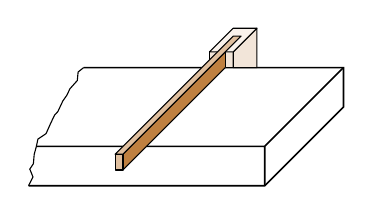
\begin{tikzpicture}[>=latex,scale=1.0]
  \draw[semithick](0,0)--(3,0)--(4,1)--(4,1.5)--(0.7,1.5);
  \draw[semithick](0.1,0.5)--(3,0.5)--(4,1.5)(3,0.5)--(3,0);
  \draw[decorate,decoration={random steps,amplitude=1pt,segment length=3pt}](0,0)--(0.1,0.5)--(0.7,1.5);
  \draw[fill=brown!20,line join=round](2.4,1.5)rectangle(2.3,1.7);
  \draw[fill=brown,line join=round](2.5,1.5)--++(0.2,0.2)--++(0,0.2)--++(-1.5,-1.5)--++(0,-0.2)--cycle;
  \draw[fill=brown!20,line join=round](2.6,1.5)rectangle(2.5,1.7);
  \draw[fill=brown!20,line join=round](2.6,1.5)--(2.6,1.7)--++(0.3,0.3)--++(0,-0.5)--cycle;
  \draw[fill=brown!10,line join=round](2.6,1.7)--(2.3,1.7)--++(0.3,0.3)--++(0.3,0)--cycle;
  \draw[fill=brown!50,line join=round](2.7,1.9)--++(-0.1,0)--++(-1.5,-1.5)--++(0.1,0)--cycle;
  \draw[fill=brown!50,line join=round](1.1,0.4)rectangle++(0.1,-0.2);
\end{tikzpicture}
\end{document}